\documentclass{beamer}

%\usetheme[framenumber,totalframenumber]{UniversiteitGent}
%\usetheme[faculty=di,framenumber,totalframenumber]{UniversiteitGent}
%\usetheme[faculty=we,usecolors,framenumber,totalframenumber]{UniversiteitGent}
%\usetheme[language=english,framenumber,totalframenumber]{AlleghenyCollege}
\usetheme{AnnArbor}
\usecolortheme{dove}

\title{CMPSC 390 \\ Bitcoin Transactions}
\author{Janyl Jumadinova \\ $ $ \\ Credit: Authors of ``Bitcoin and Cryptocurrency Technologies"}
\date{January 28, 2021}

\long\def\omitit#1{}

\usepackage{hyperref}
\hypersetup{
    colorlinks=true,
    linkcolor=blue,
    filecolor=magenta,      
    urlcolor=cyan,
}

\begin{document}

\begin{frame}
  \titlepage
\end{frame}

%%%%%%%%%%%% Slide %%%%%%%%%%%%%%%%%%%%%%%%%%%%%%%%%%%%%%%%%%%%%%%%%%%
\begin{frame}
  \frametitle{Where we left off ... }
  Bitcoin consensus
  \begin{itemize}
  	\item Append-only ledger. 
  	\item Decentralized consensus.
  	\item Miners to validate transactions.
  \end{itemize}
  \pause
  assuming a currency exists to motivate miners!
\end{frame}
%%%%%%%%%%%% Slide %%%%%%%%%%%%%%%%%%%%%%%%%%%%%%%%%%%%%%%%%%%%%%%%%%%
\begin{frame}
  \frametitle{UTXO Model}
  \begin{itemize}
  	\item Unspent Transaction Output Model. 
  	\pause
  	\item Transactions map inputs to outputs.
  	\item An account holds a set of \textcolor{brown}{)}
  		\begin{itemize}
  			\item Transactions contain signature of fund's owner.
  			\item Spending bitcoin is redeeming previous transaction outputs.
  		\end{itemize}
  \end{itemize}
\end{frame}

%%%%%%%%%%%% Slide %%%%%%%%%%%%%%%%%%%%%%%%%%%%%%%%%%%%%%%%%%%%%%%%%%%
\begin{frame}
  \frametitle{An account-based ledger (not Bitcoin)}
  
\centering
	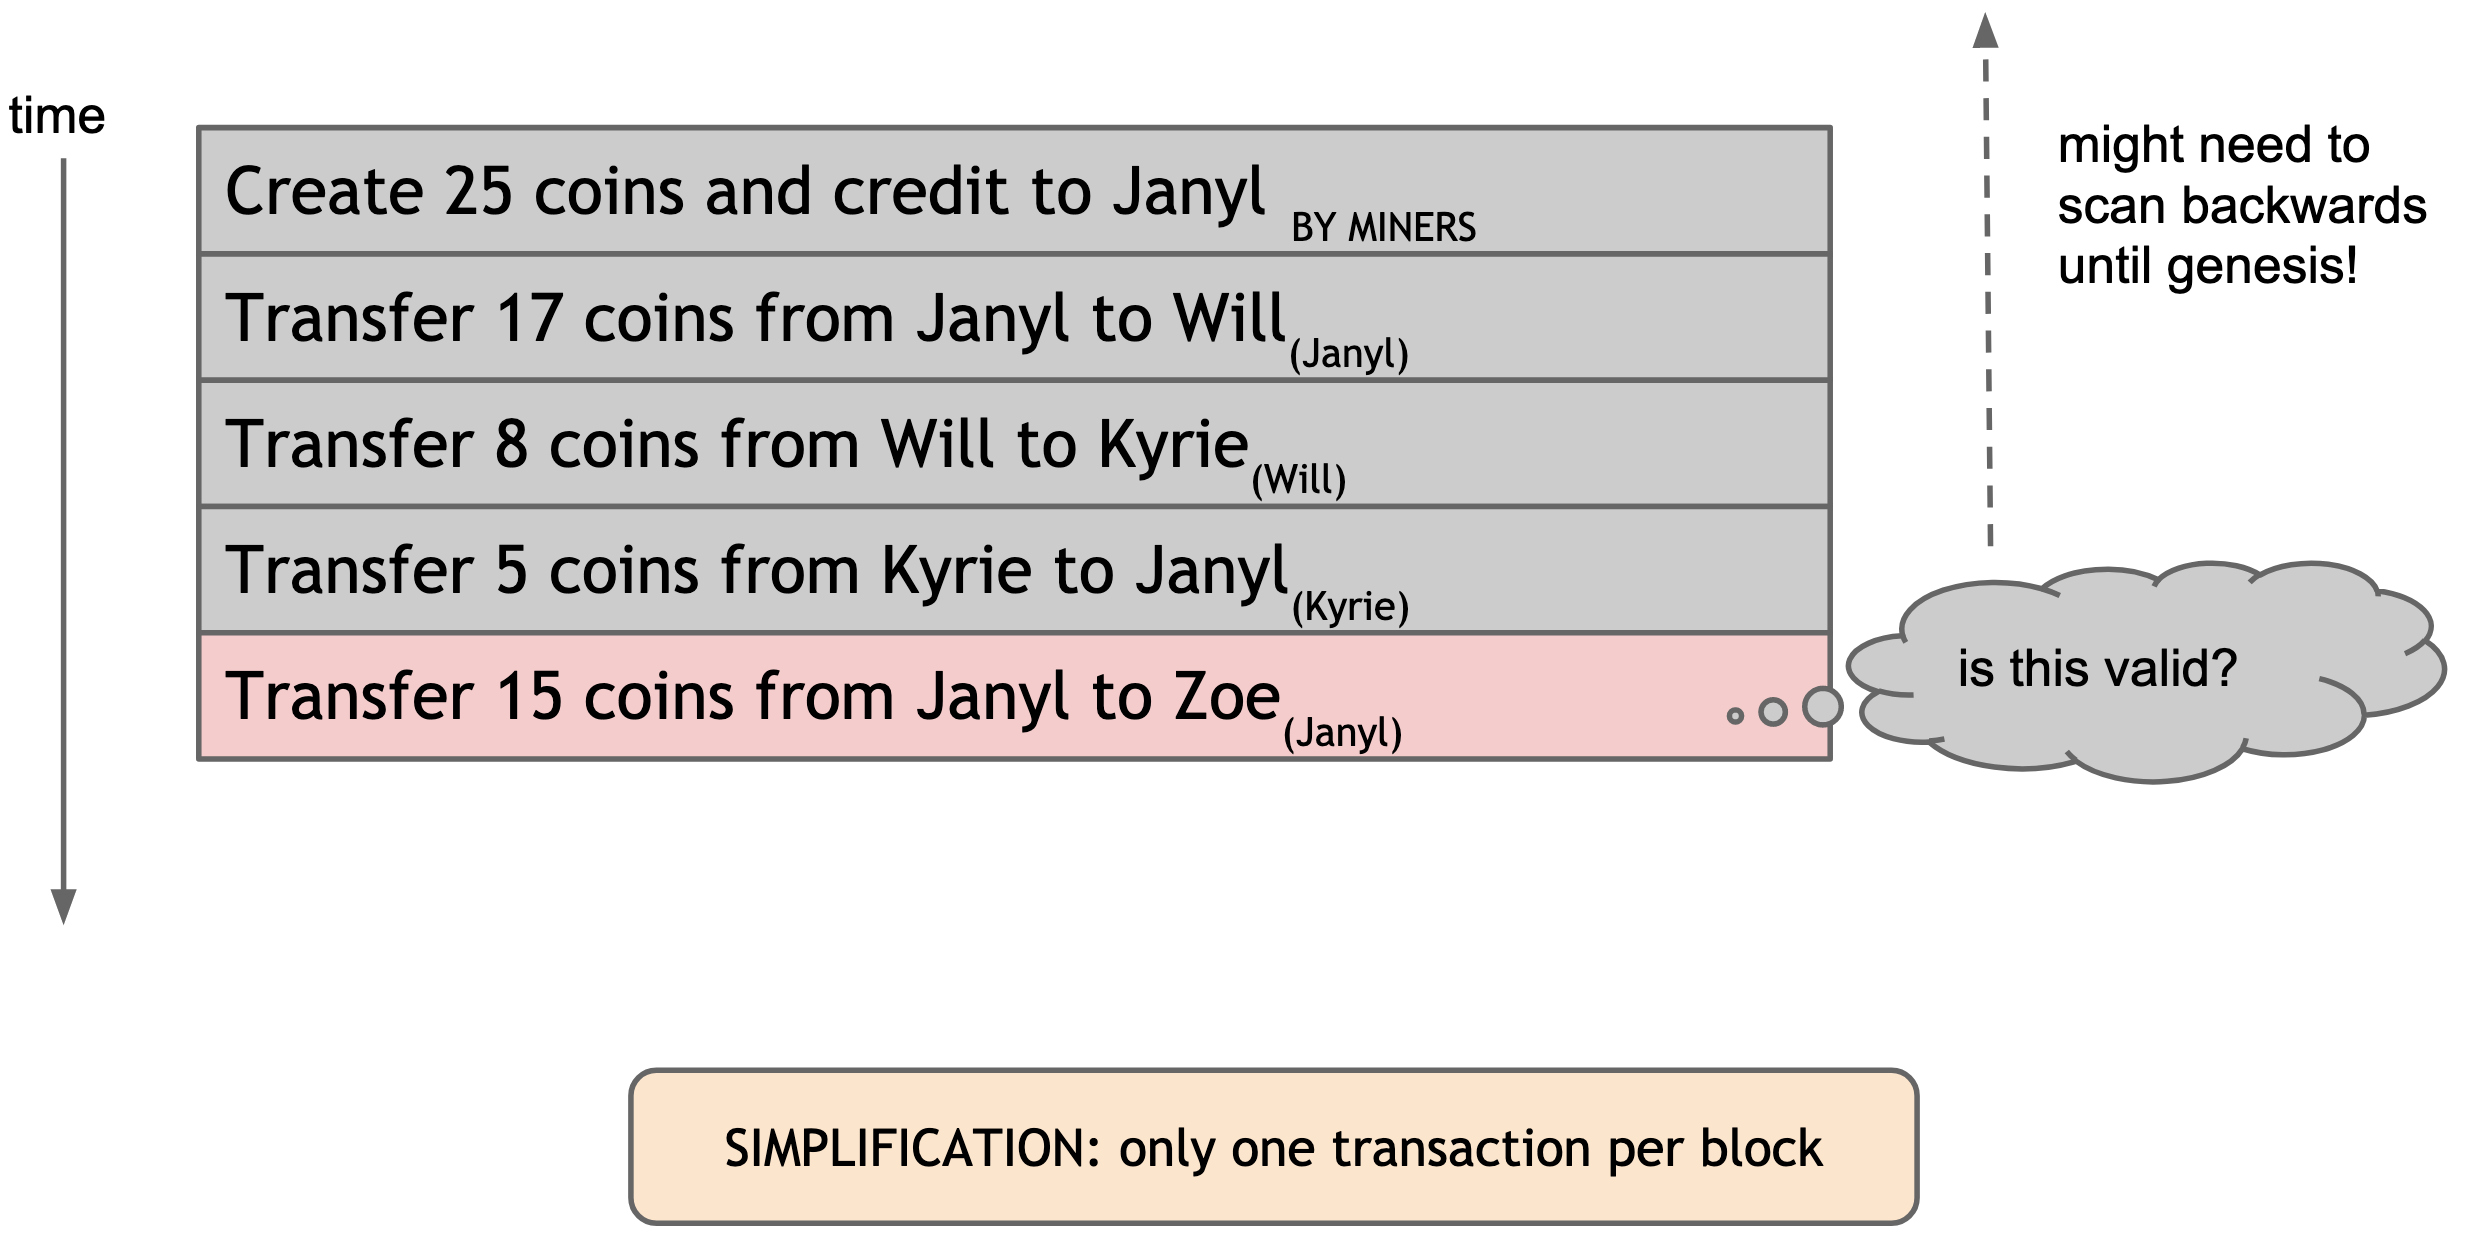
\includegraphics[scale=0.25]{1-1}
\end{frame}

%%%%%%%%%%%% Slide %%%%%%%%%%%%%%%%%%%%%%%%%%%%%%%%%%%%%%%%%%%%%%%%%%%
\begin{frame}
  \frametitle{Transaction-based ledger (Bitcoin)}
  
\centering
	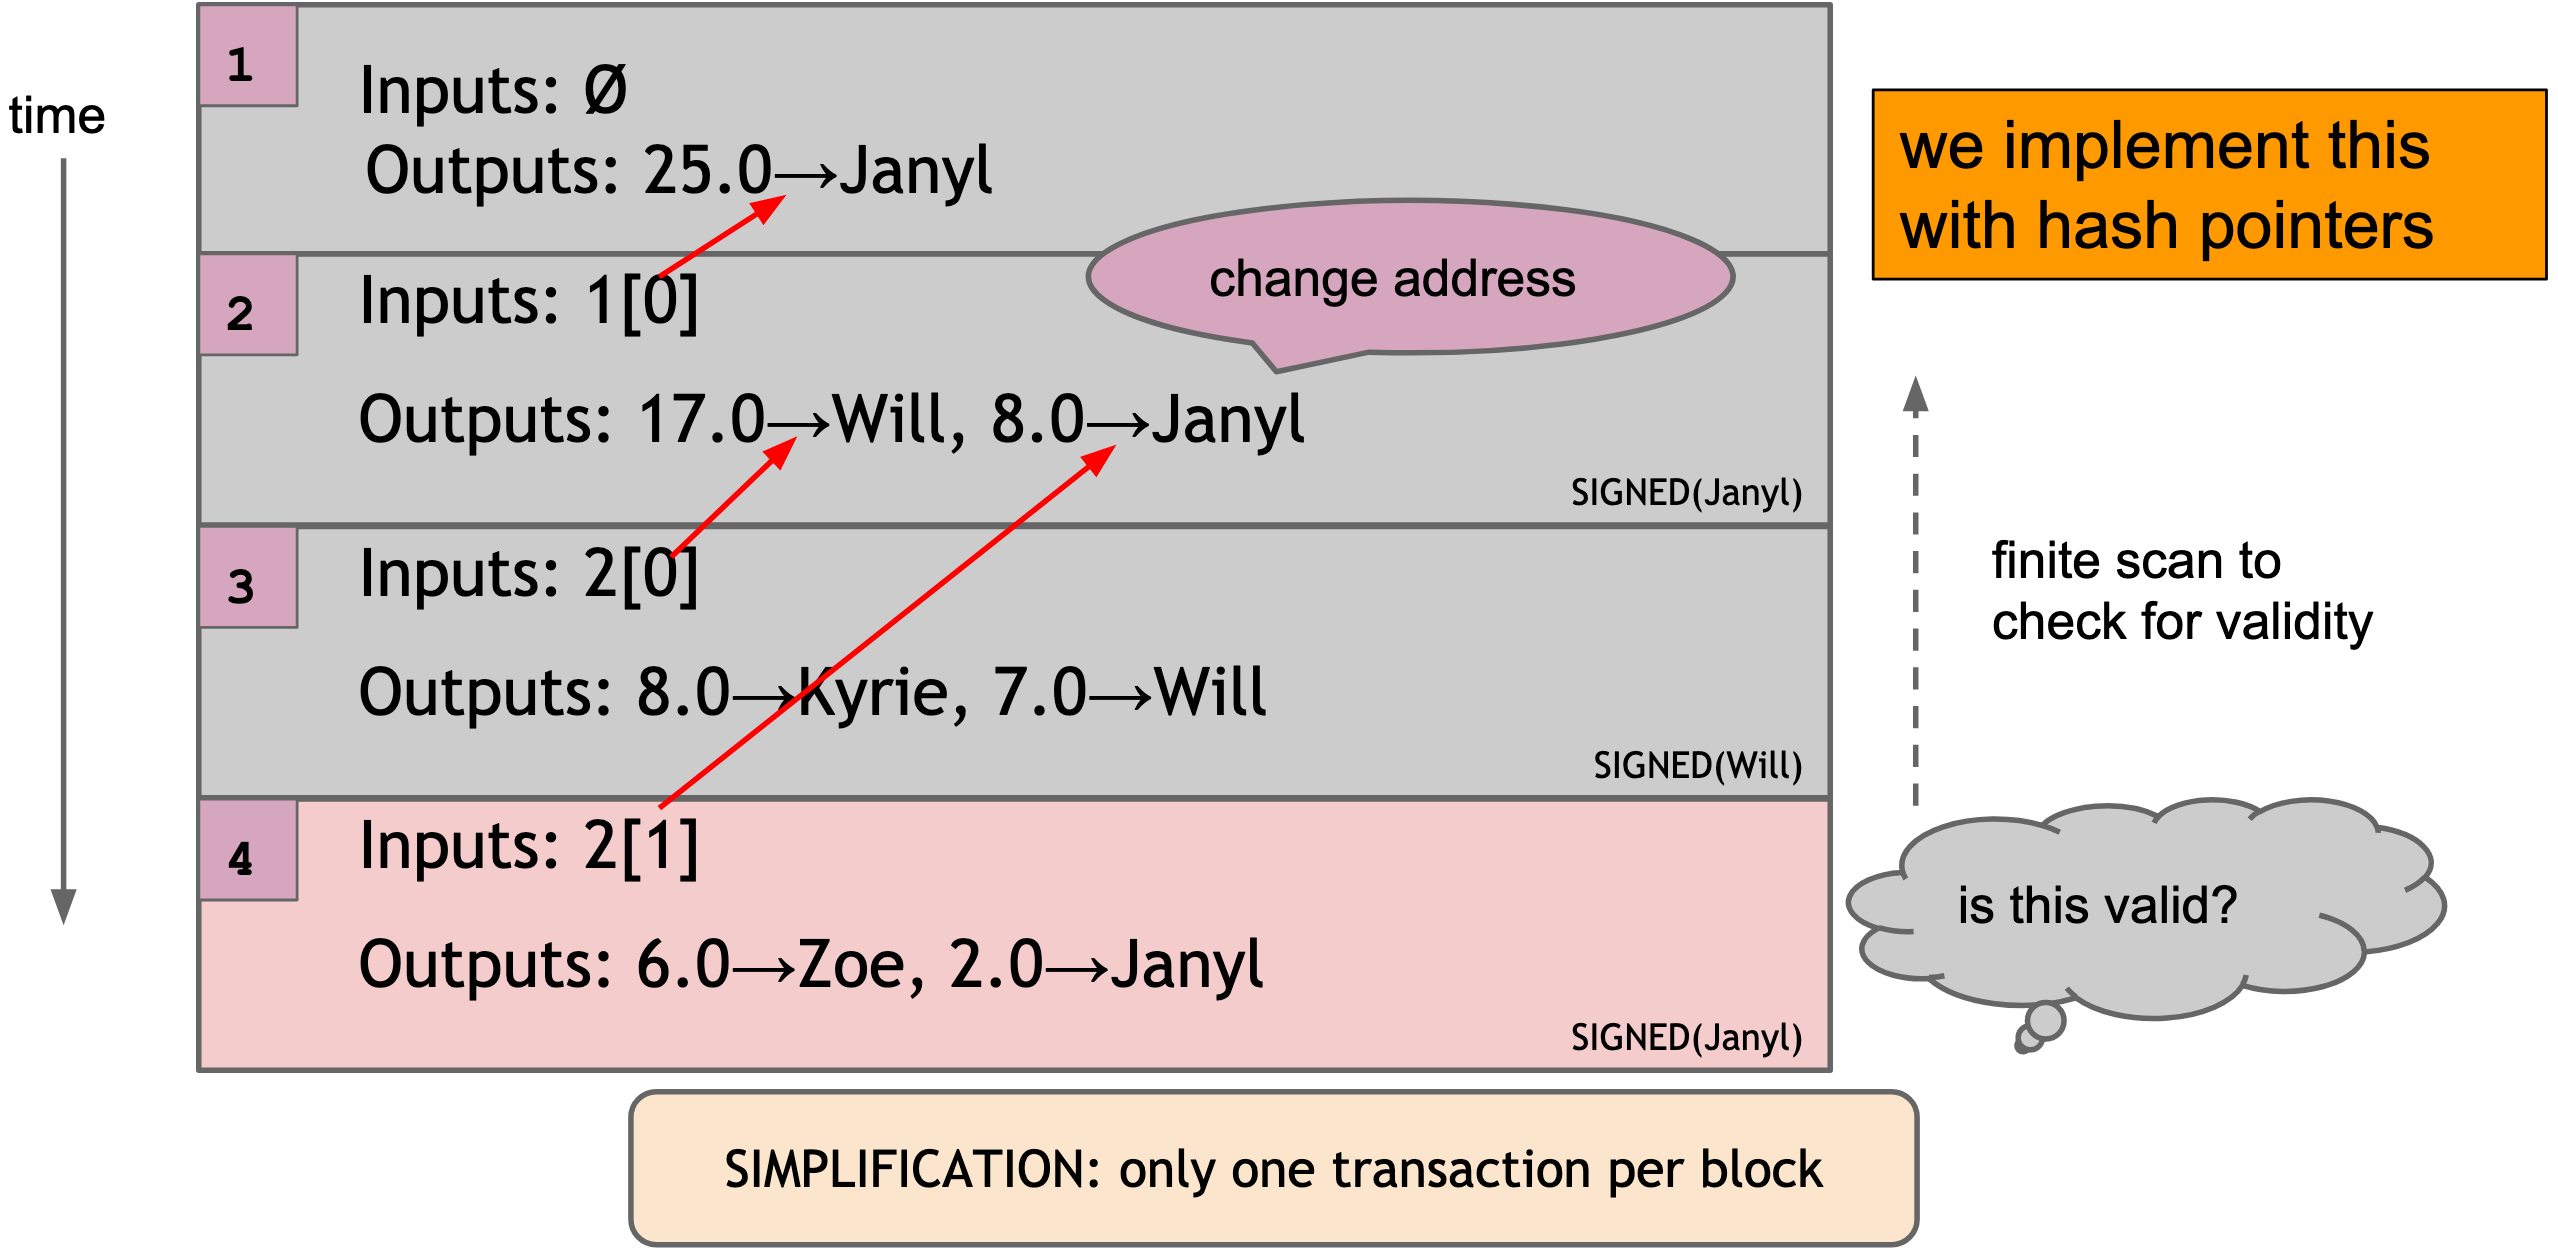
\includegraphics[scale=0.28]{2-1}
\end{frame}

%%%%%%%%%%%% Slide %%%%%%%%%%%%%%%%%%%%%%%%%%%%%%%%%%%%%%%%%%%%%%%%%%%
\begin{frame}
  \frametitle{Merging Value}
  
\centering
	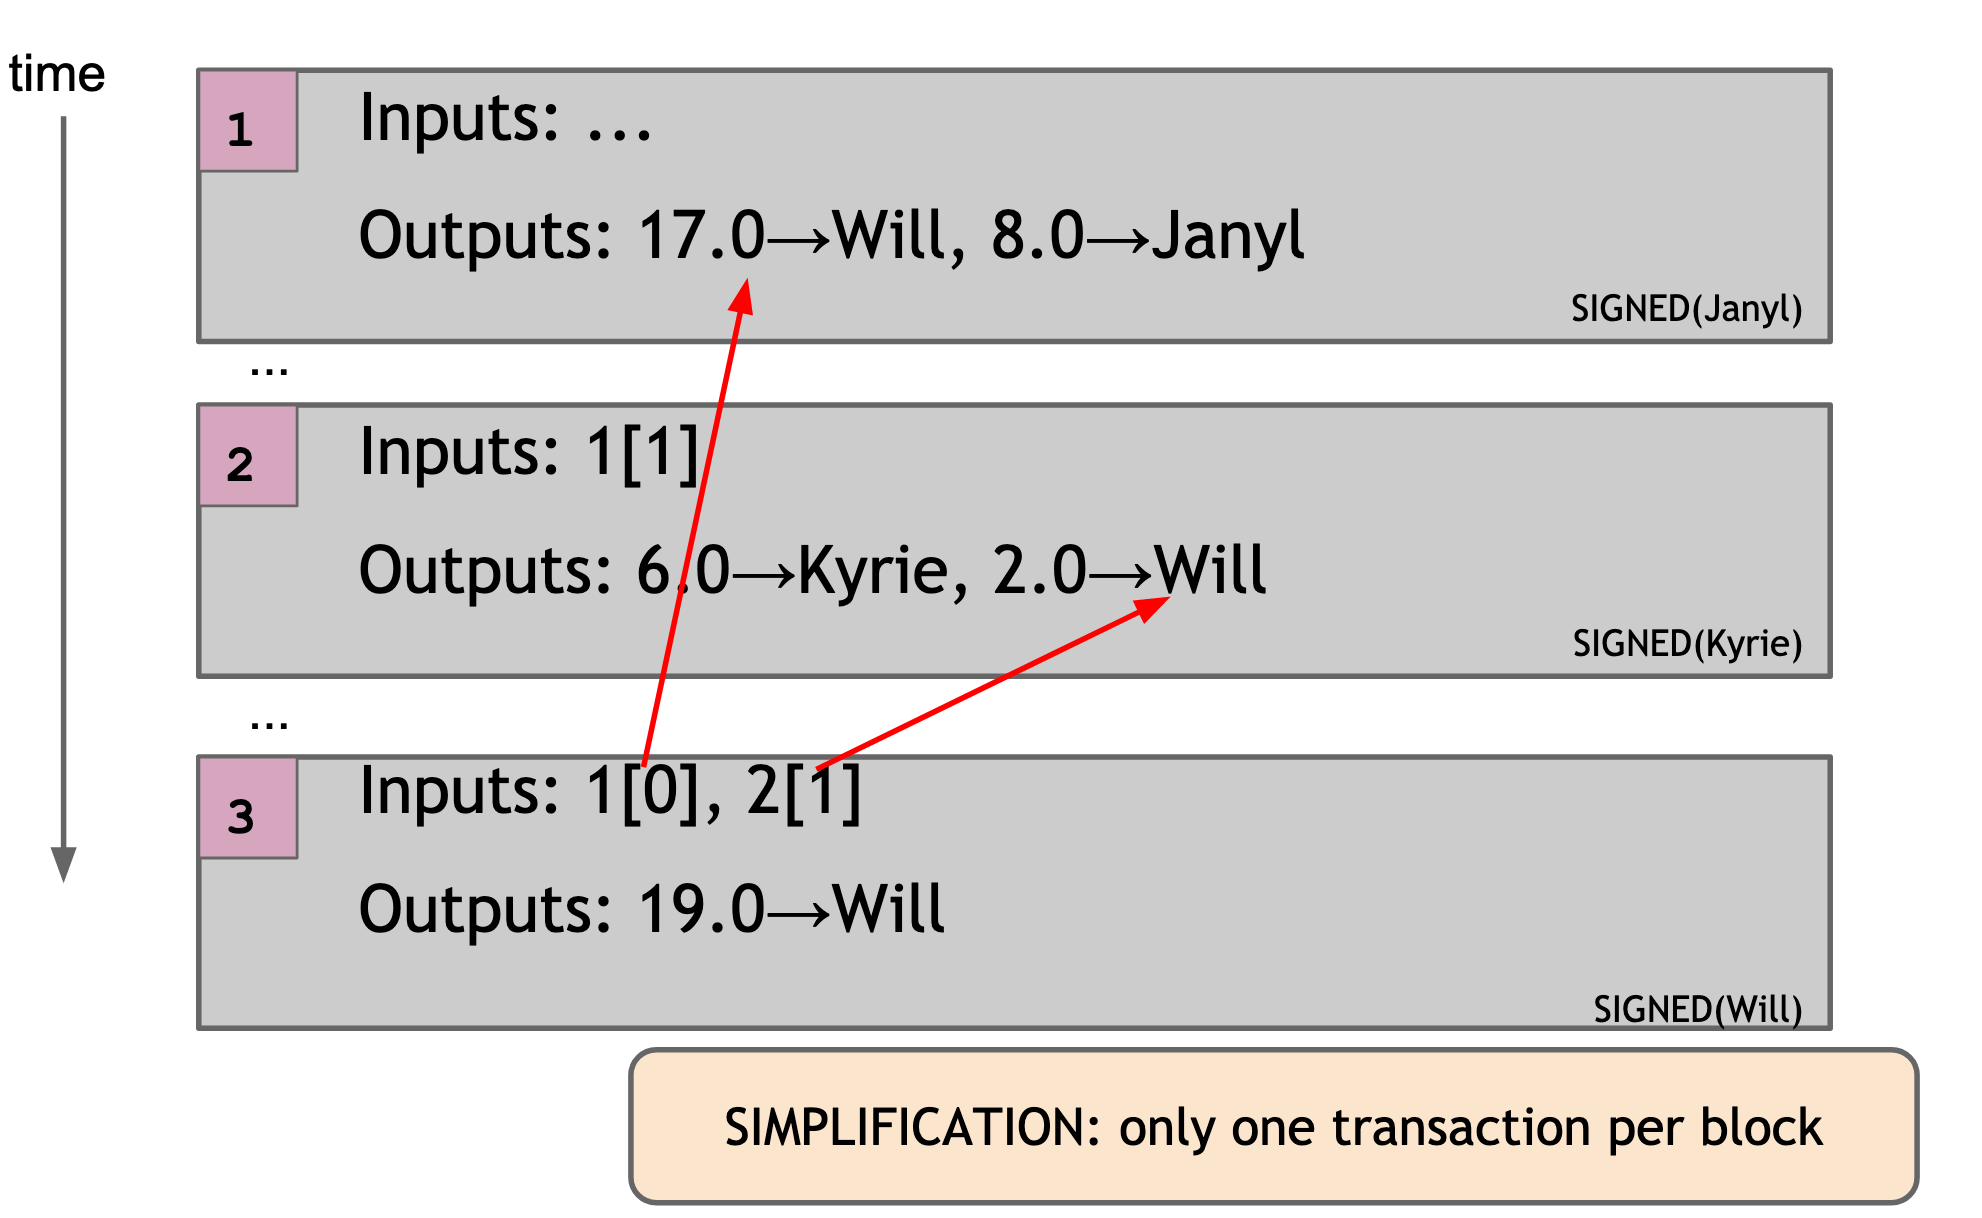
\includegraphics[scale=0.3]{3-1}
\end{frame}
%%%%%%%%%%%% Slide %%%%%%%%%%%%%%%%%%%%%%%%%%%%%%%%%%%%%%%%%%%%%%%%%%%
\begin{frame}
  \frametitle{Joint Payments}
  
\centering
	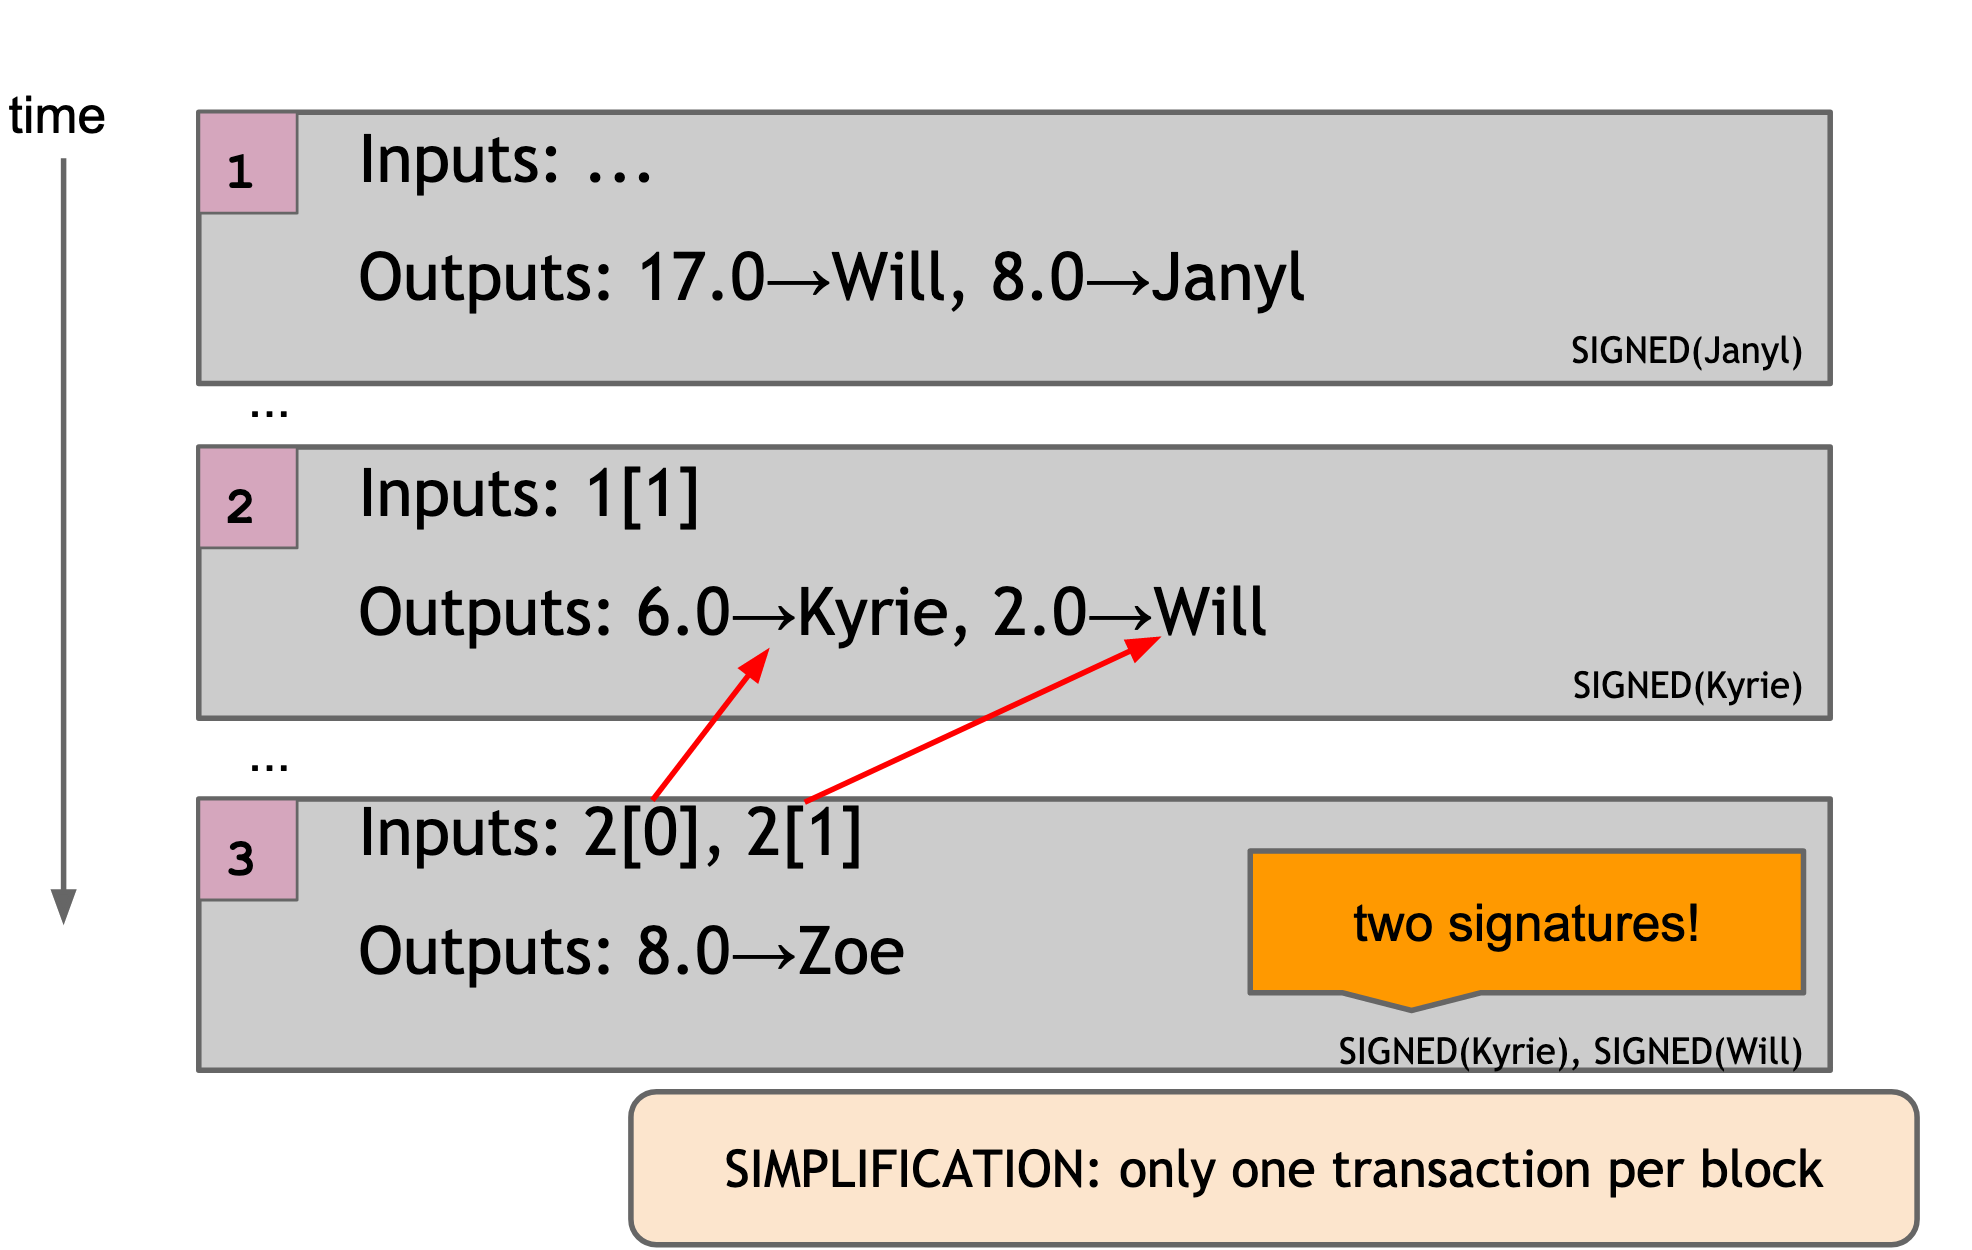
\includegraphics[scale=0.3]{4-1}
\end{frame}
%%%%%%%%%%%% Slide %%%%%%%%%%%%%%%%%%%%%%%%%%%%%%%%%%%%%%%%%%%%%%%%%%%
\begin{frame}
  \frametitle{Bitcoin transaction}

\centering
	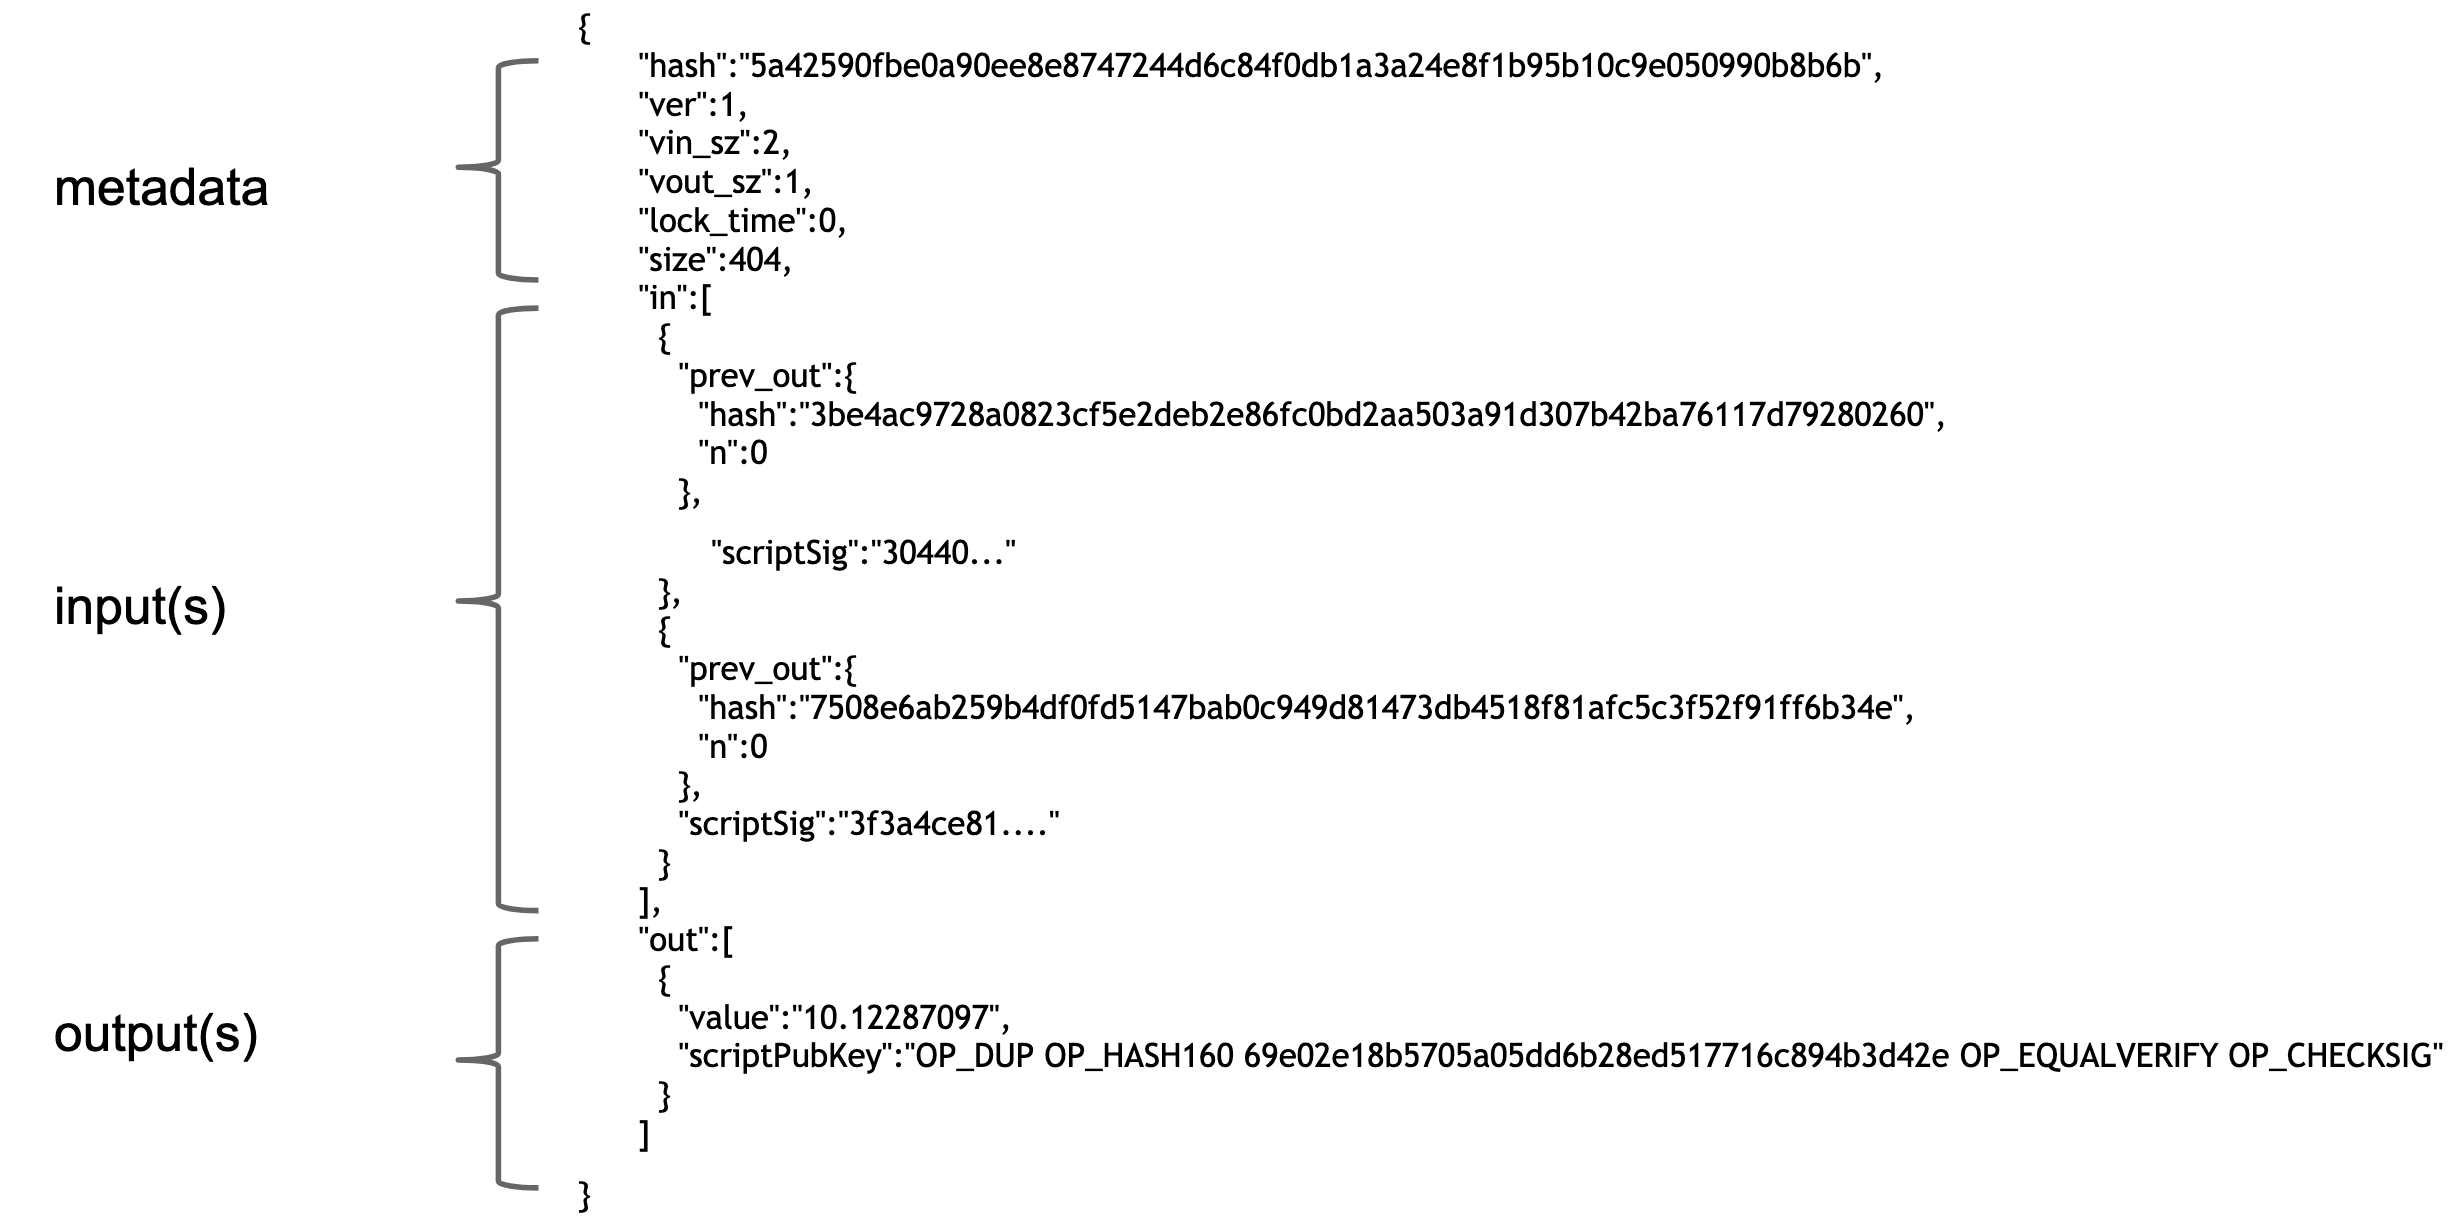
\includegraphics[scale=0.3]{transaction}
\end{frame}
%%%%%%%%%%%% Slide %%%%%%%%%%%%%%%%%%%%%%%%%%%%%%%%%%%%%%%%%%%%%%%%%%%
\begin{frame}
  \frametitle{Bitcoin transaction: metadata}

\centering
	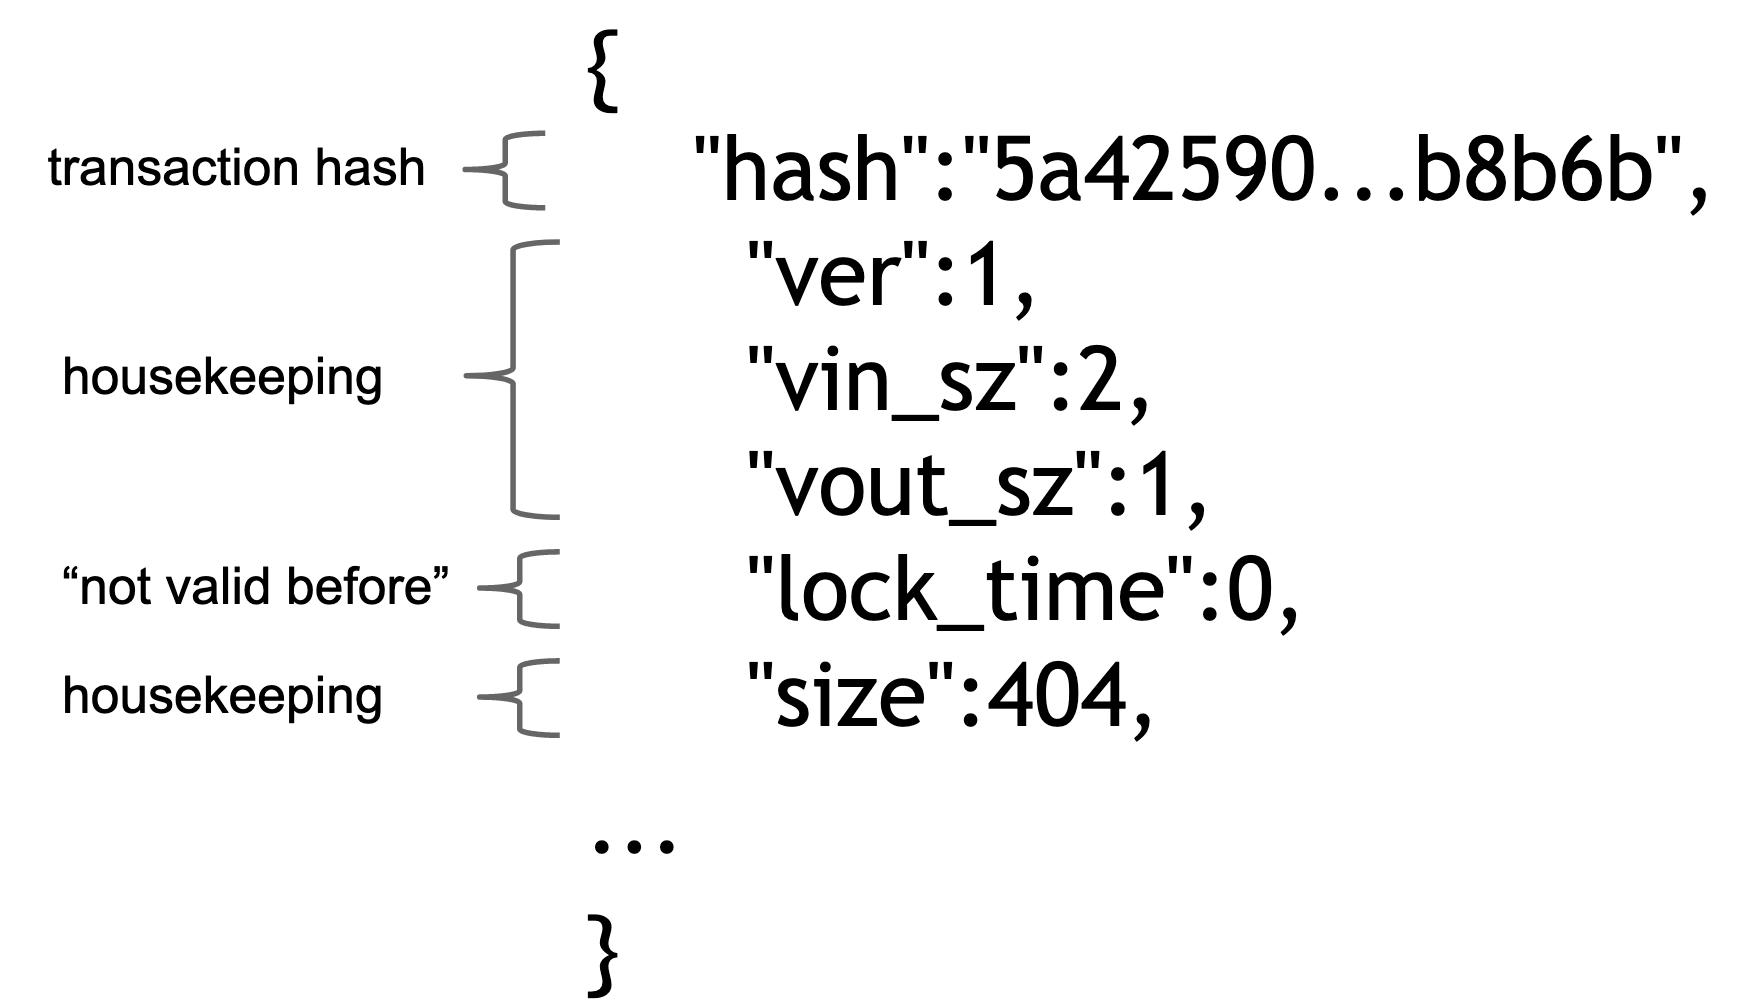
\includegraphics[scale=0.3]{4}
\end{frame}
%%%%%%%%%%%% Slide %%%%%%%%%%%%%%%%%%%%%%%%%%%%%%%%%%%%%%%%%%%%%%%%%%%
\begin{frame}
  \frametitle{Bitcoin transaction: inputs}

\centering
	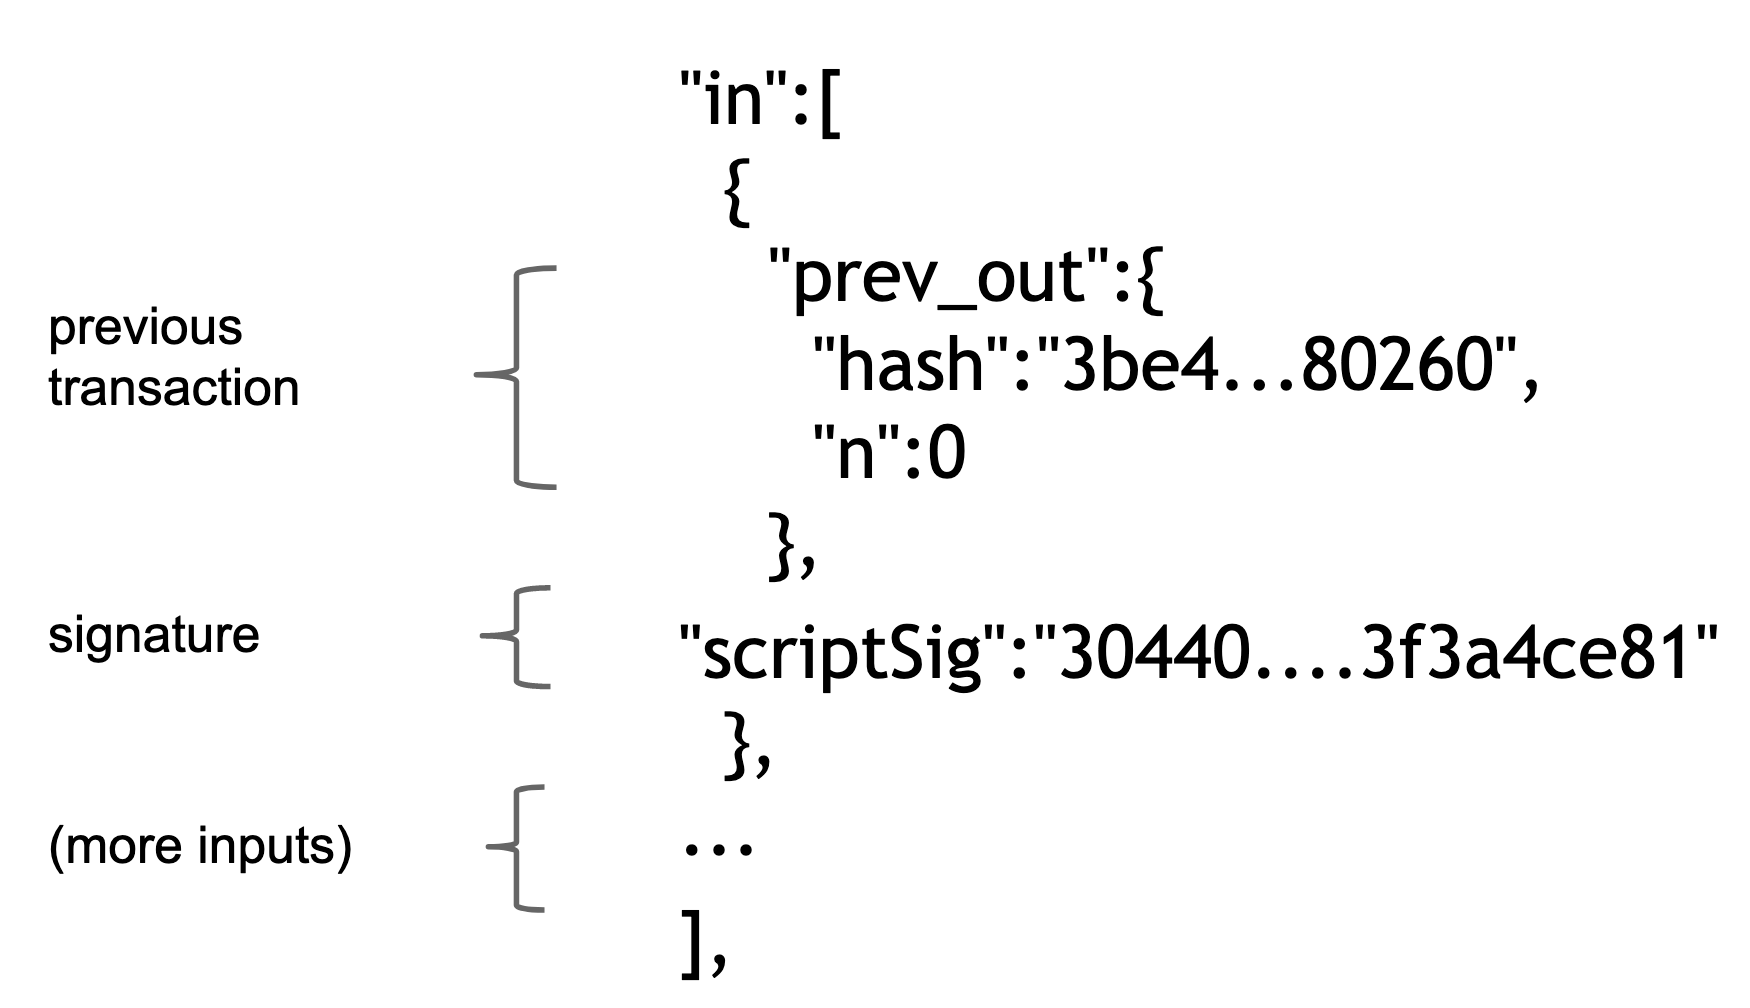
\includegraphics[scale=0.3]{5}
\end{frame}
%%%%%%%%%%%% Slide %%%%%%%%%%%%%%%%%%%%%%%%%%%%%%%%%%%%%%%%%%%%%%%%%%%
\begin{frame}
  \frametitle{Bitcoin transaction: outputs}

\centering
	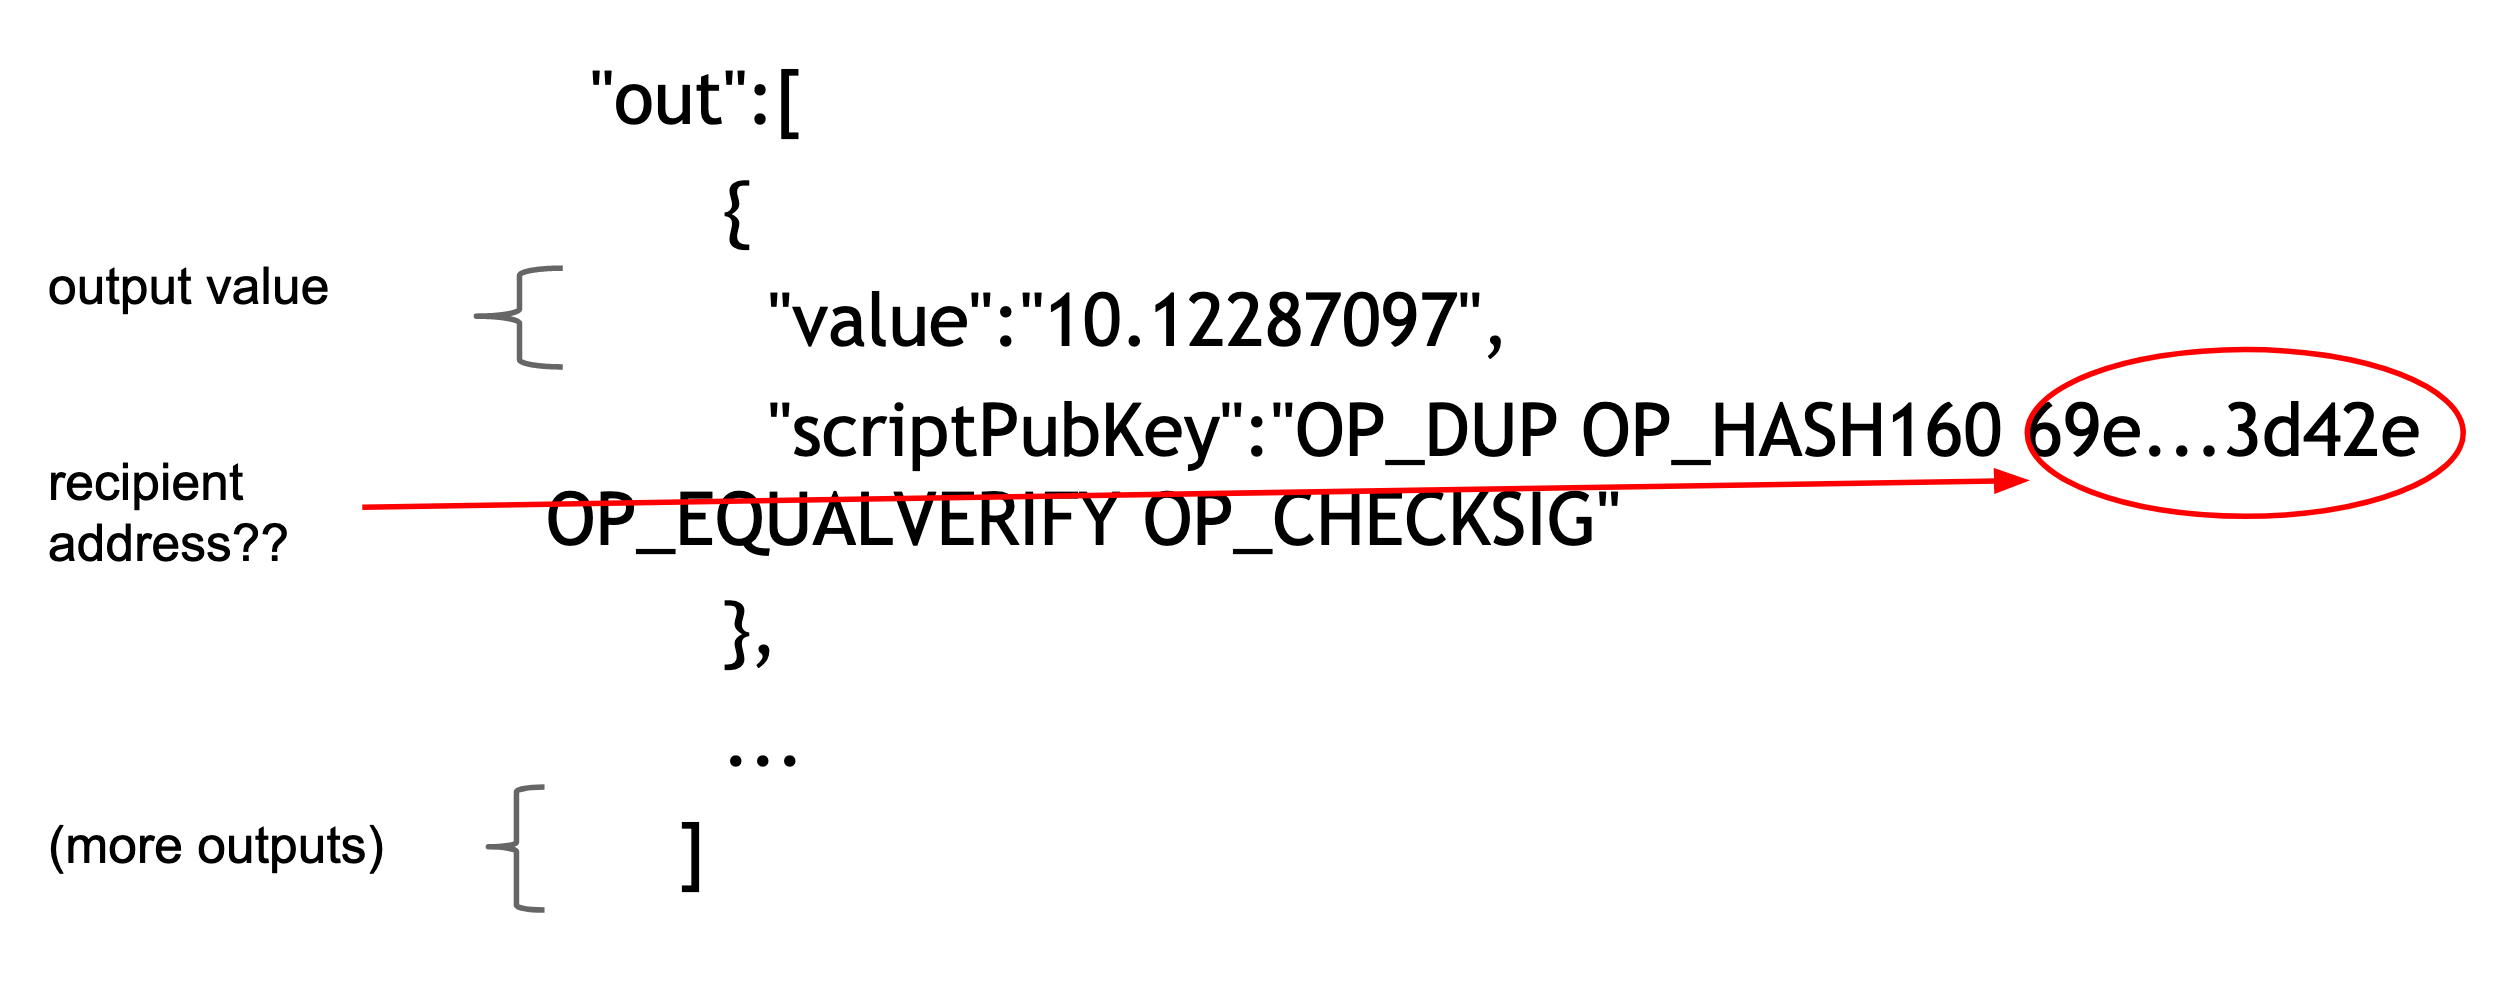
\includegraphics[scale=0.28]{6}
\end{frame}
%%%%%%%%%%%% Slide %%%%%%%%%%%%%%%%%%%%%%%%%%%%%%%%%%%%%%%%%%%%%%%%%%%
\begin{frame}
  \frametitle{Bitcoin Script}
  
  \begin{itemize}
  	\item Output ``addresses'' are actually \textcolor{brown}{scripts}.
  	\pause
  	\item Input ``addresses'' are also scripts.
  \end{itemize}
  \pause
  
  \centering
	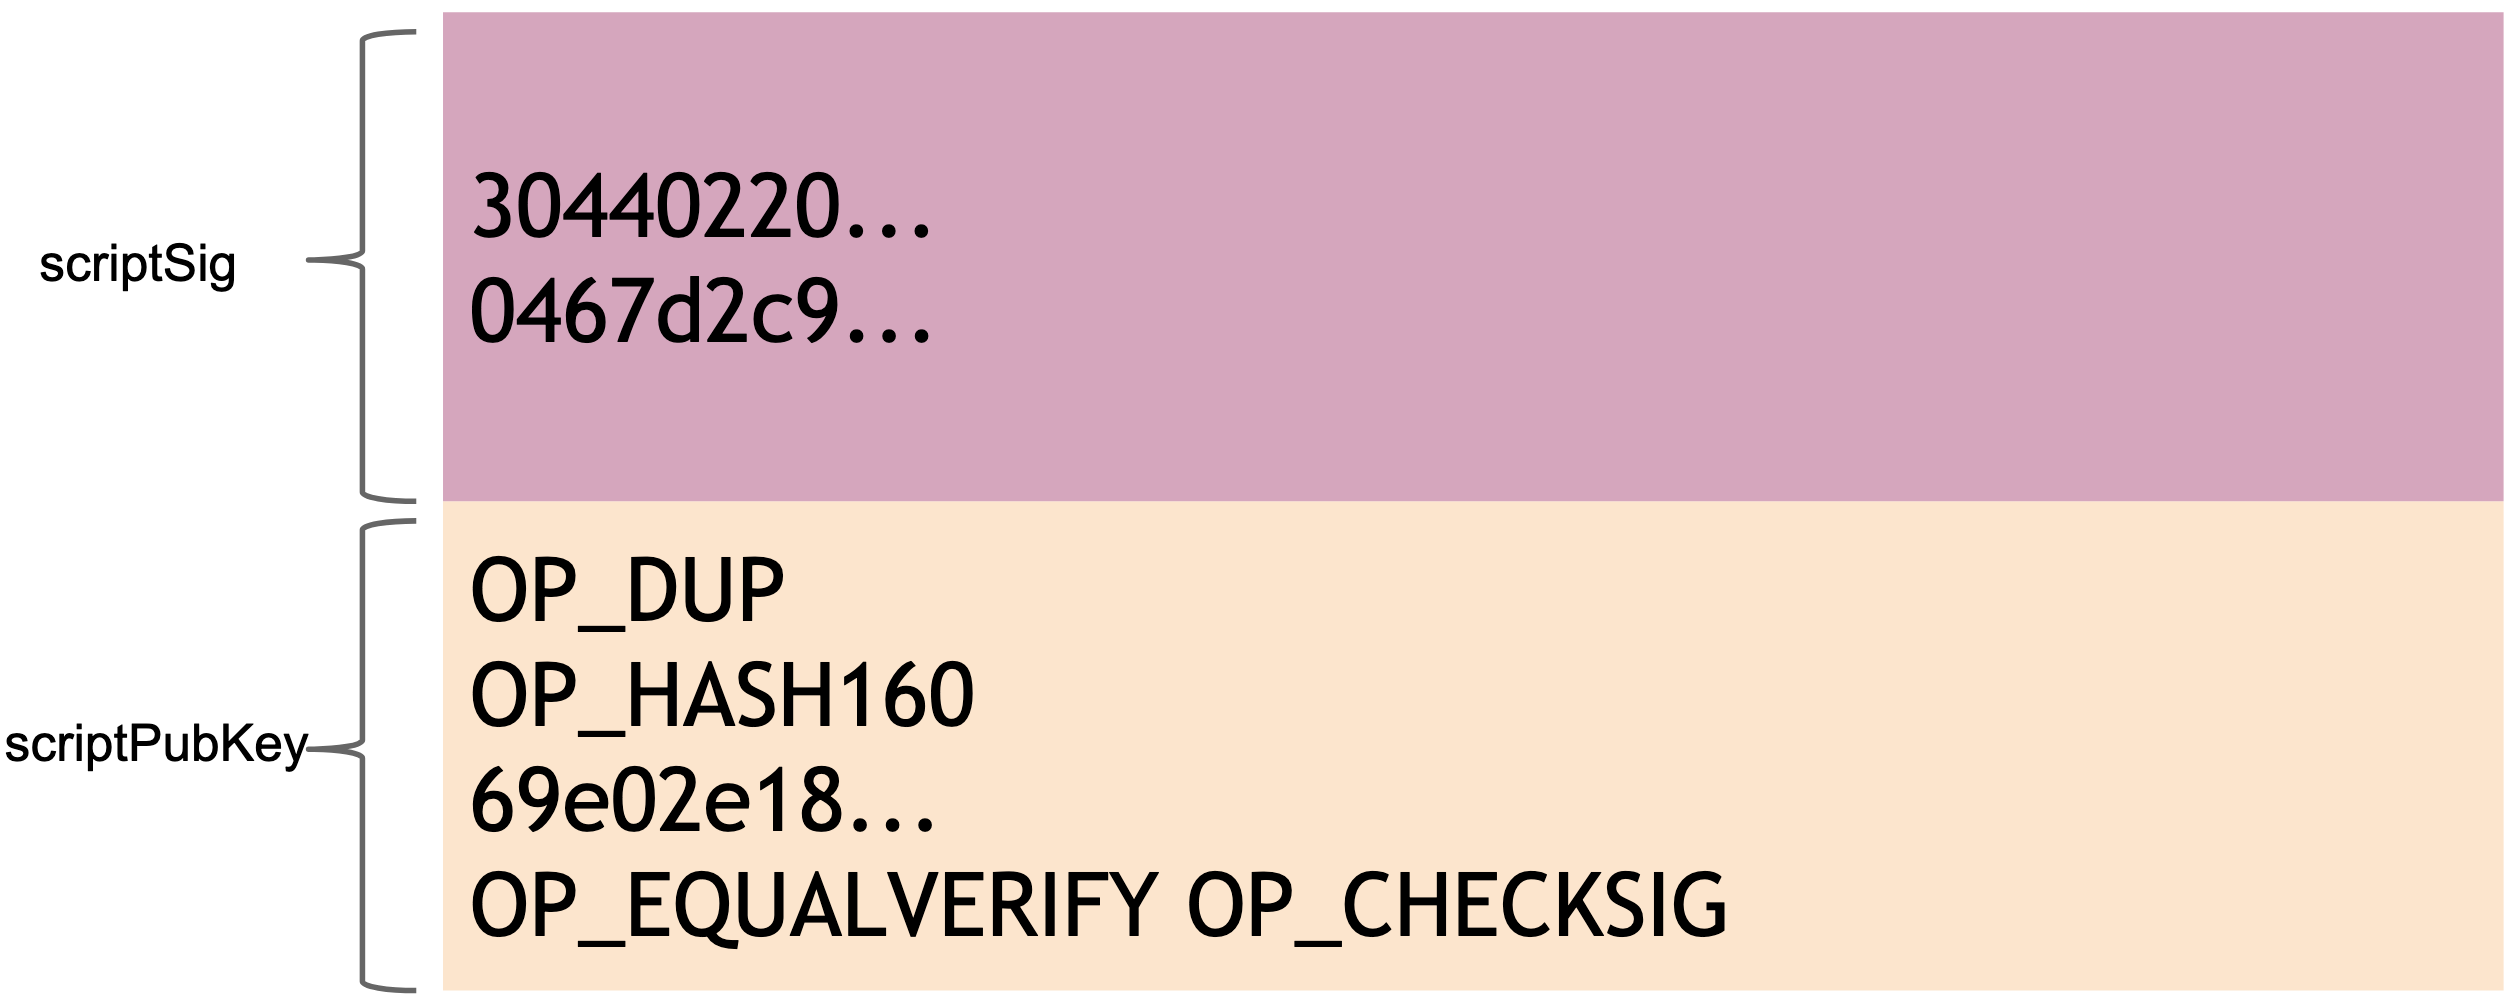
\includegraphics[scale=0.3]{scripts}
\end{frame}

%%%%%%%%%%%% Slide %%%%%%%%%%%%%%%%%%%%%%%%%%%%%%%%%%%%%%%%%%%%%%%%%%%
\begin{frame}
  \frametitle{Bitcoin Scripting Language (``Script'')}
  
  \begin{itemize}
  	\item Built for Bitcoin (inspired by Forth). 
	\item Simple, compact.
	\item Support for cryptography.
	\item Stack-based.
	\item Limits on time/memory.
	\item No looping.

  \end{itemize}
  
\end{frame}
%%%%%%%%%%%% Slide %%%%%%%%%%%%%%%%%%%%%%%%%%%%%%%%%%%%%%%%%%%%%%%%%%%
\begin{frame}[fragile]
  \frametitle{Bitcoin Script Example}
  
  \begin{verbatim}
<sig> <pubKey> OP_DUP OP_HASH160 <pubKeyHash?> 
																OP_EQUALVERIFY OP_CHECKSIG
  \end{verbatim}
  
  \pause
  \centering
	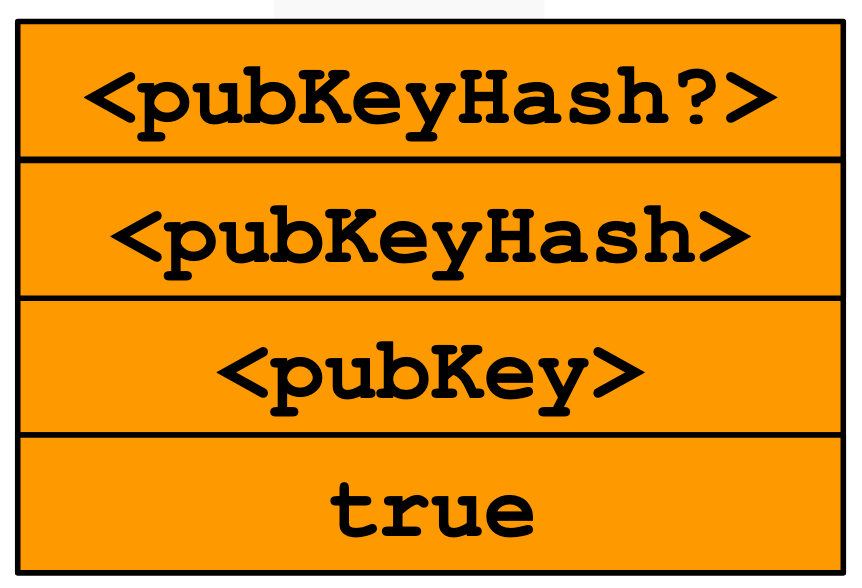
\includegraphics[scale=0.3]{7}
\end{frame}
%%%%%%%%%%%% Slide %%%%%%%%%%%%%%%%%%%%%%%%%%%%%%%%%%%%%%%%%%%%%%%%%%%
\begin{frame}
  \frametitle{Bitcoin Scripting instructions}
  256 opcodes total
  \begin{itemize}
  	\item Arithmetic
	\item If/then
	\item Logic/data handling \pause
	\item Hashes. Signature verification. Multi-signature verification
  \end{itemize}
  
\end{frame}
%%%%%%%%%%%% Slide %%%%%%%%%%%%%%%%%%%%%%%%%%%%%%%%%%%%%%%%%%%%%%%%%%%
\begin{frame}
  \frametitle{Bitcoin Blocks}
  
  \centering
	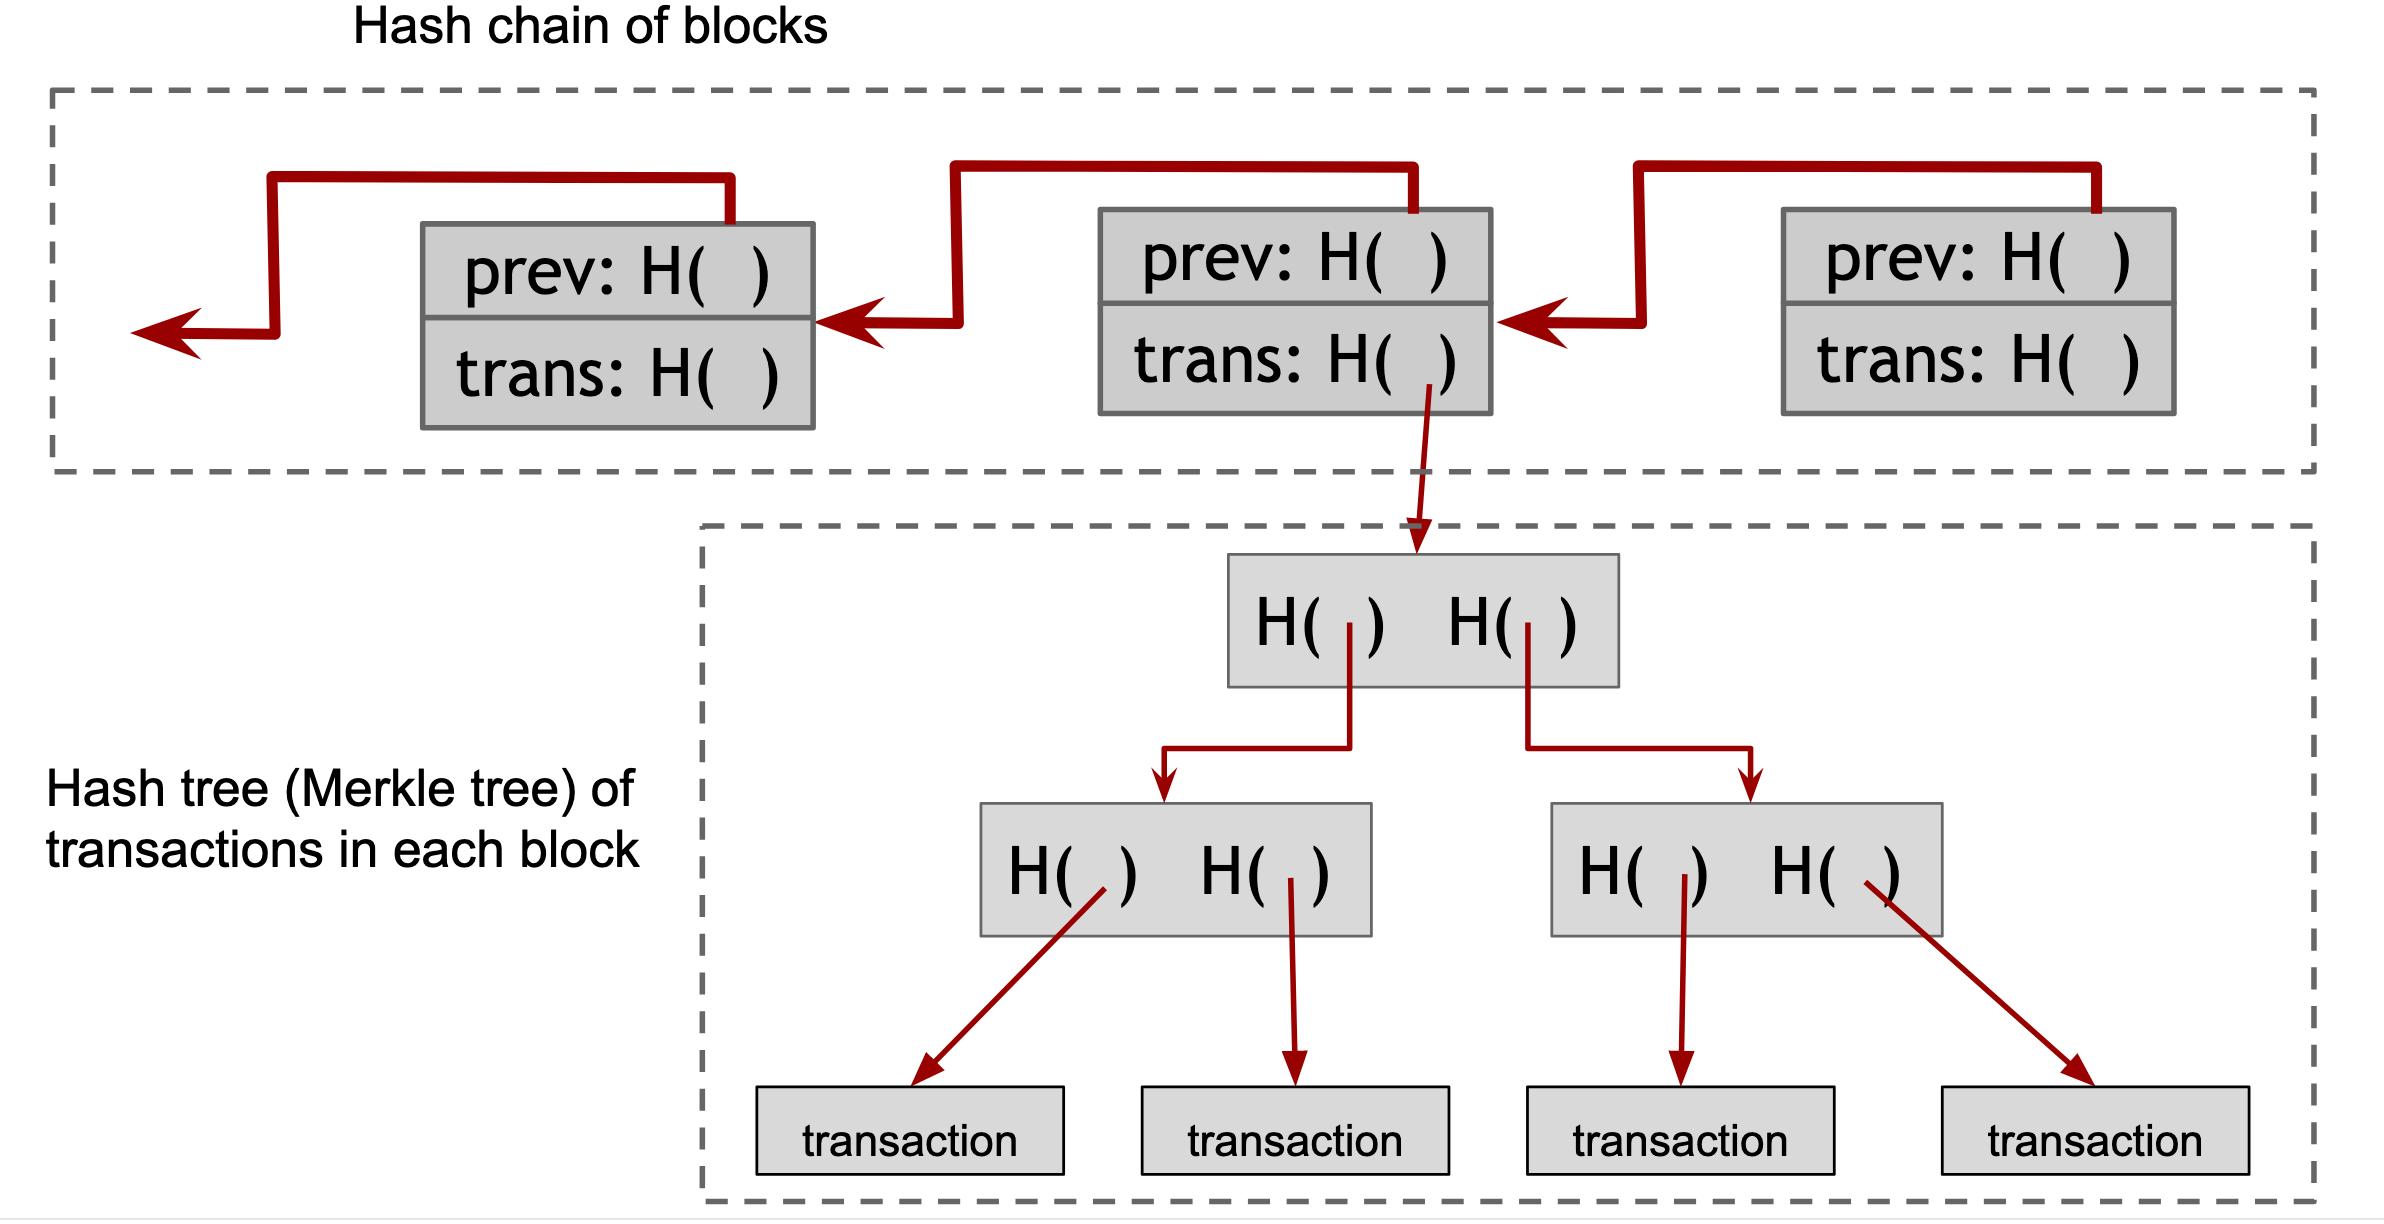
\includegraphics[scale=0.29]{blockchain}
  
\end{frame}
%%%%%%%%%%%% Slide %%%%%%%%%%%%%%%%%%%%%%%%%%%%%%%%%%%%%%%%%%%%%%%%%%%
\begin{frame}
  \frametitle{Bitcoin Blocks}
  
  \centering
	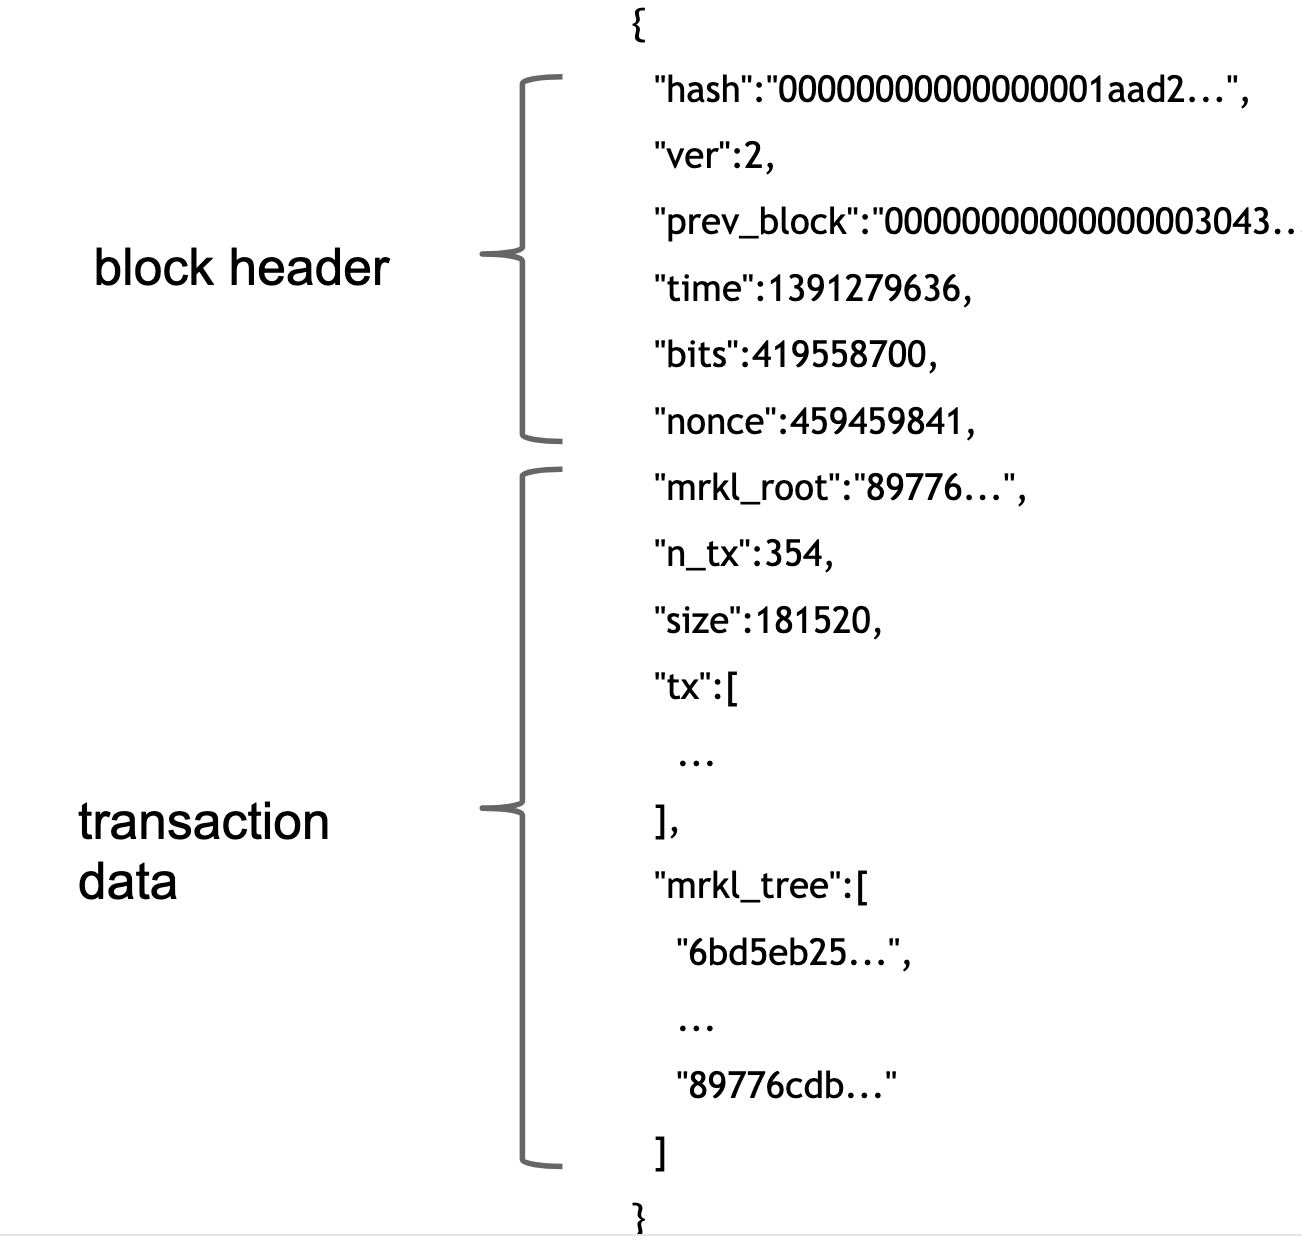
\includegraphics[scale=0.3]{block1}
  
\end{frame}
%%%%%%%%%%%% Slide %%%%%%%%%%%%%%%%%%%%%%%%%%%%%%%%%%%%%%%%%%%%%%%%%%%
\begin{frame}
  \frametitle{Bitcoin Blocks}
  
  \centering
	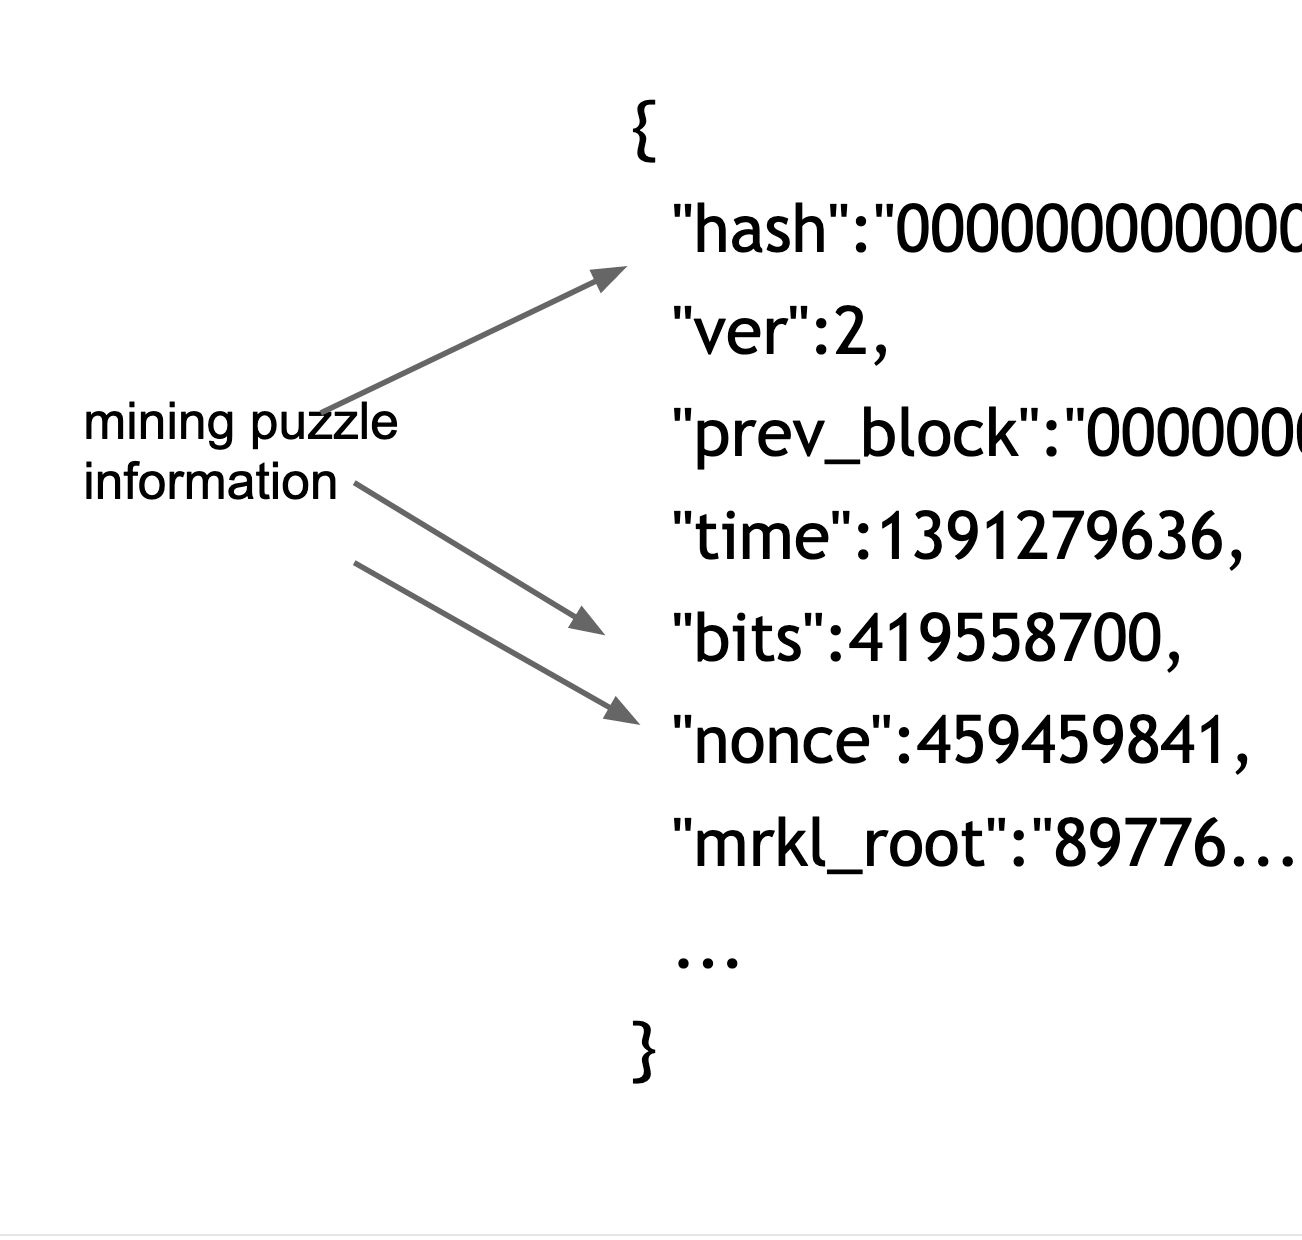
\includegraphics[scale=0.3]{block2}
  
\end{frame}
%%%%%%%%%%%% Slide %%%%%%%%%%%%%%%%%%%%%%%%%%%%%%%%%%%%%%%%%%%%%%%%%%%
\begin{frame}
  \frametitle{Bitcoin Blocks}
  
  \centering
	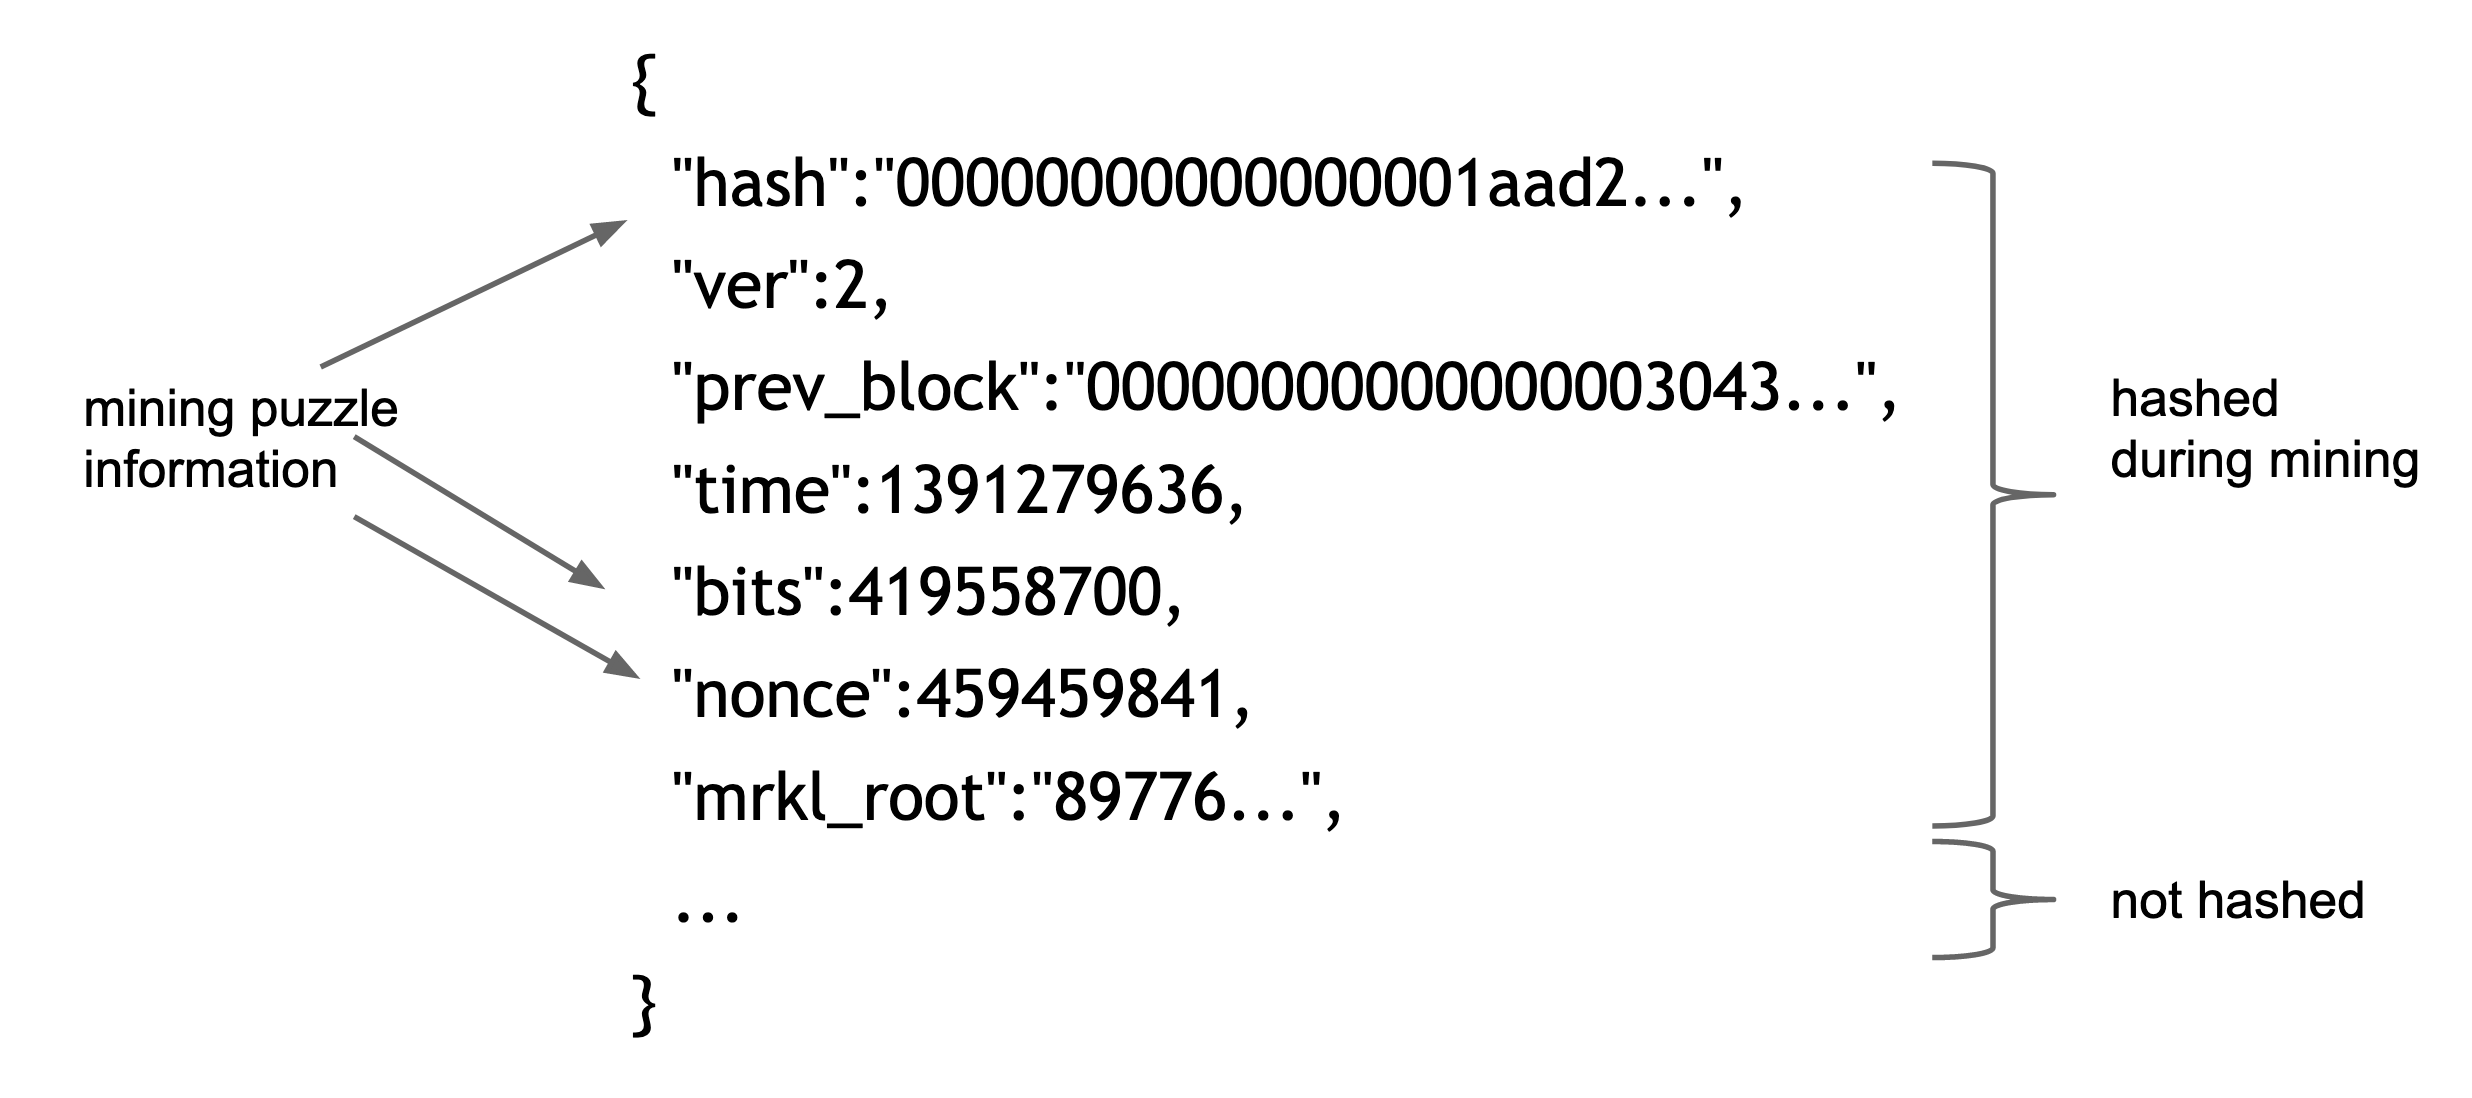
\includegraphics[scale=0.28]{block3}
  
\end{frame}
%%%%%%%%%%%% Slide %%%%%%%%%%%%%%%%%%%%%%%%%%%%%%%%%%%%%%%%%%%%%%%%%%%


%%%%%%%%%%%% Slide %%%%%%%%%%%%%%%%%%%%%%%%%%%%%%%%%%%%%%%%%%%%%%%%%%%
\end{document}
